\documentclass[11pt]{article}
\usepackage[margin=.78in]{geometry}
\usepackage{amsmath,amssymb,graphicx,hyperref,booktabs}
\setlength{\parindent}{0pt}\setlength{\parskip}{6pt}
\begin{document}
{\LARGE Next experiment: complete target-chord decomposition}\\
2026-11-05\quad Execution-design follow-on to merged PR3438

\textbf{Status.} Proposed construction and finite experiment. No native scientific
run, proof build, identity certificate or measured advantage. PCC statement
\texttt{PCC-20261105-7179e4} has no signed verification. [pcc:unverified]

For actual $R=(a,b)$ on $y^2=x^3+Ax+B$, the proposed line through $-R$ is
$L_l(X)=l(X-a)-b$. Let
\[
q_l=X^2-sX+p,\quad s=l^2-a,\quad p=al^2+2bl+a^2+A.
\]
Proof target: $X^3+AX+B-L_l(X)^2=(X-a)q_l(X)$ using the actual target
equation. For $F_B=X^3-c_1X^2+c_2X-c_3$, prove its remainder is $UX+V$,
\[
U=s^2-p-c_1s+c_2,\quad V=(c_1-s)p-c_3,\quad W=V+aU.
\]
The proposed $U,W$ chart has quartic/cubic degrees, with special leading
cancellations recorded honestly. These are proof obligations, not checked
degree or runtime results. [pcc:unverified]

\begin{center}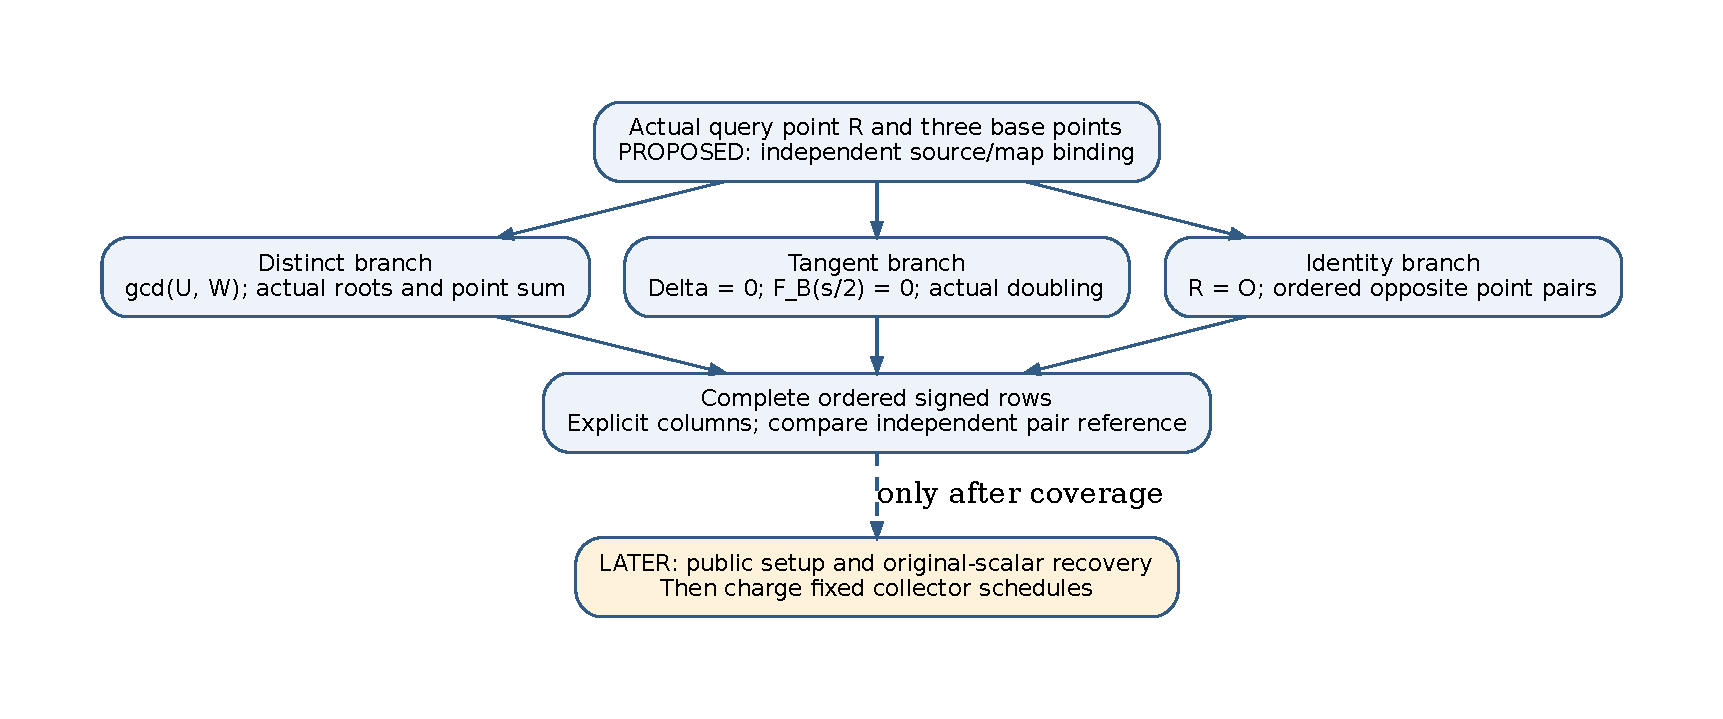
\includegraphics[width=\linewidth,height=2.72in,keepaspectratio]{branches.pdf}\end{center}

\textbf{The missing branch matters.} A repeated-root quadratic need not divide
the square-free base polynomial. Keep $\Delta=s^2-4p=0$ and
$F_B(s/2)=0$ for the diagonal branch, with actual point and doubling checks.
Handle $R=O$ separately. Prove coverage, including coincident intersections,
signs and the nonzero denominator, before algebraic admission. [pcc:unverified]

\small Background: \href{https://eprint.iacr.org/2004/031}{Semaev, 2004/031};
\href{https://arxiv.org/html/1503.08001v2}{Kosters--Yeo, sections 2 and 4--5}.
The current atlas already records eliminants, membership and transported-base
mechanisms. This design makes no invention claim. [pcc:unverified]
\clearpage
{\LARGE Finite census, then original-source recovery}

\textbf{Actual proposed fixture.} $E/\mathbf F_{37}:y^2=x^3+7x+19$,
nonsquare $d=35$ twist $T:y^2=x^3+28x+33$,
$P=(1,8)\mapsto U=(32,29)$, subgroup order19. Rebind and recheck historical
coordinate $\Phi$ and inverse $I=[10]D$ on the actual cyclic subgroups.
Relation coefficients use $\mathbf F_{19}$, distinct from the curve field.
No new registry or generic map claim. [pcc:unverified]

\begin{center}\begin{tabular}{ll}\toprule
Planned factor & Complete declared population\\\midrule
Base policy & All 84 size-three policies per role\\
Role & Main, native twist, matched, pulled-back\\
Query & All 19 subgroup points, including identity\\
Cells per instrument & $84\times4\times19=6,384$ planned\\
Nonidentity cells & 6,048, repeating 18 public points\\\bottomrule
\end{tabular}\end{center}
These are repeated policy/query/control records, not thousands of distinct
DLP challenges. Rust candidate and separate C++ arithmetic reference/auditor
are unimplemented. A/A repeats the candidate for deterministic replay.
No full-census data exists. [pcc:unverified]

\textbf{Pass condition.} Every required cell completes with zero missing or
extra ordered signed rows. Plant distinct, tangent and identity relations
through the production path first. False roots, omitted branches, wrong
columns/source/map/rank/witness or missing queries must reject changed,
rehashed payloads with no receipt. A missed positive control invalidates the
instrument; a timeout is incomplete coverage. [pcc:unverified]

\textbf{Degree/work records.} Keep univariate degrees, exact witnesses,
construction, extraction, field/group/map and row work separately. A gcd has
no Macaulay matrix degree: record null, not zero. Any later matrix comparison
uses the same original ideal and expanded original-input witnesses. No
intrinsic regularity, equal-weight counter sum or speed result is implied.
[pcc:unverified]

\textbf{Next acceptance.} After coverage, freeze separate cold setup and all 18
original-target recoveries per policy/role. Derive public base logs only from
admitted relations; retain blocked setups and every failed shift. Check the
scalar on original $E/P$. Then test fixed collector schedules against the
entire source-policy frontier, charging both calls, maps and setup. Complete
identical per-query row sets cannot yield strict union complementarity.
The trace-variable construction remains queued. [pcc:unverified]

\textbf{Launch dependency.} Exact checkpoint-only prefix approval is pending
for the new execution branch. The official uploading gate must succeed before
any scientific/proof launch. Native/proof/analysis instruments and source hashes
are still missing; the canonical protocol is DRAFT. Use at most two existing
local workers, 600-second stages and one window no longer than 3600 seconds.
No paid resources or arbitrary result uploads.

\small See the adjacent algorithm, protocol and launch documents.\\
This diagram has no measured data; old quantitative graphs and benchmarks
remain unchanged. [pcc:unverified]
\end{document}
